\begin{itemize}
    \item It is also worth observing that the non-ambiguous interval for the arccos is \(\pi\) and not \(2\pi\). Hence, the estimate of \(f_0\) is non-ambiguous of \(B=F_c/2\) rather than \(2B =F_c\) as it is for the Periodogram.
    \item From the next figures we derive that the MM estimator is not efficient. In fact, its MSE is far from the CRB. However, the \textbf{computational complexity} is much lower than that of the ML estimator, so in some applications it can be preferred, thanks to its reduced computational complexity. This typically happens in applications where the processing must be done in real-time.
\begin{figure}[H]
    \centering
    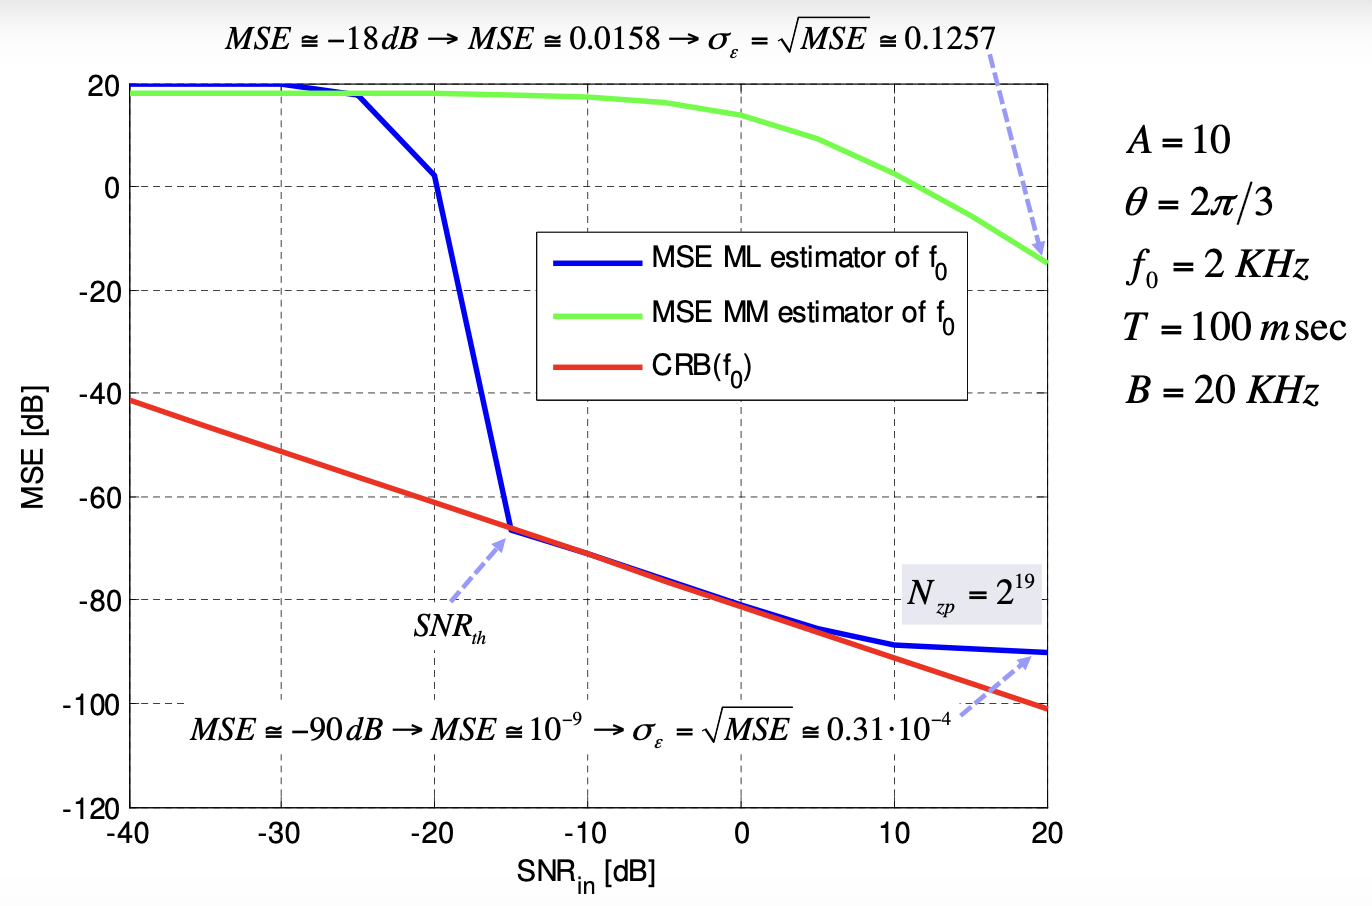
\includegraphics[width=0.6\linewidth]{Image/pdf 4/55.MSE_1.png}
    \label{fig:placeholder}
\end{figure}
    \begin{figure}[H]
        \centering
        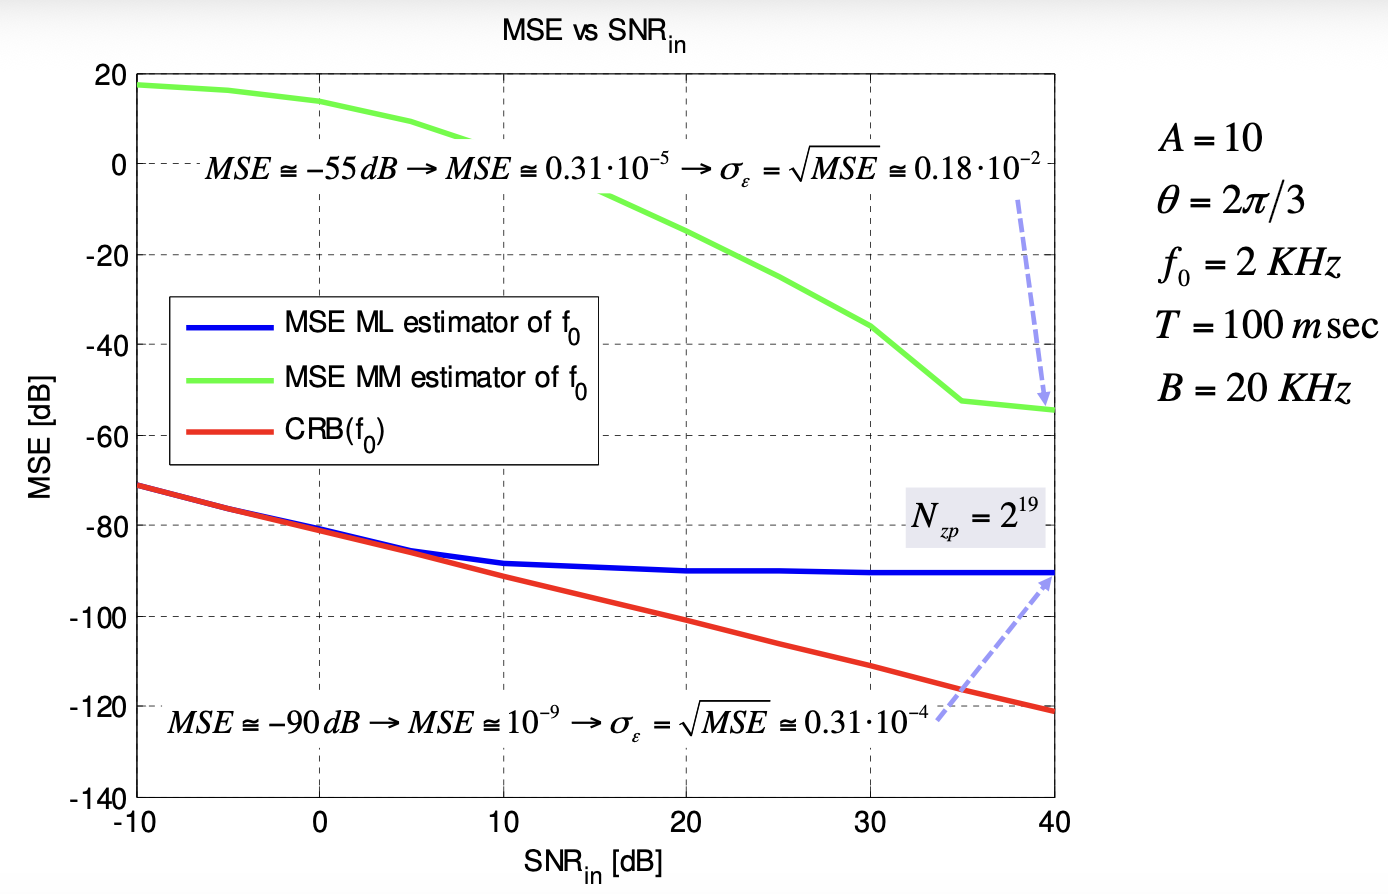
\includegraphics[width=0.6\linewidth]{Image/pdf 4/56.MSE_2.png}
        \label{fig:placeholder}
    \end{figure}
\begin{figure}[H]
    \centering
    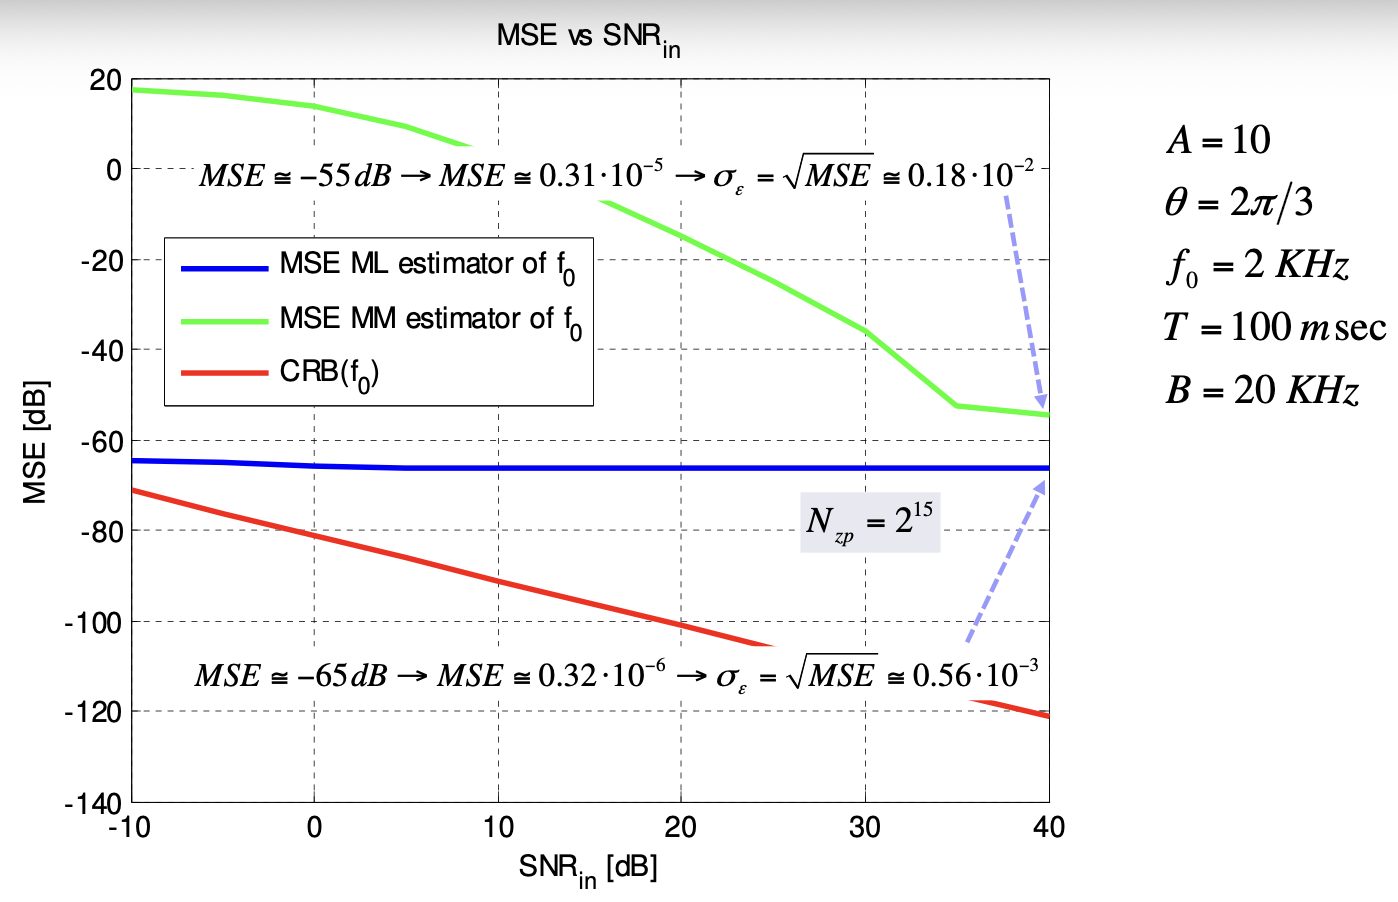
\includegraphics[width=0.6\linewidth]{Image/pdf 4/57.MSE_3.png}
    \label{fig:placeholder}
\end{figure}

    \item \underline{\textbf{Summary on the estimation of the frequency of a cosinusoidal signal}}:
    \begin{itemize}
        \item \textbf{ML estimate}: efficient if \(SNR>SNR_{th}\): the algorithm is not in closed-form; the estimate requires the search for the maximum of the \textbf{Periodogram}; computational complexity : medium-high; non-ambiguous estimation interval: \(2B=F_c\).
        \item \textbf{MM estimate}: need for \(SNR_{in}\gg 1\), not efficient, the algorithm is in closed-form; low computational complexity, to be preferred when we need a fast estimate; non-ambiguous estimation interval : \(B=F_c/2\).
        \item The estimation accuracy of the MM estimator can be improved by exploiting the sample estimates of the ACF at more lags.
    \end{itemize}

\end{itemize}
\subsection{ML Estimate of the Parameters of a Multi-component Signal}

\[
X(t) = s(t) + W(t), \qquad t \in [0,T)
\]
\[
s(t) = A_{1} \cos\bigl(2\pi f_{1} t + \theta_{1}\bigr)
      + A_{2} \cos\bigl(2\pi f_{2} t + \theta_{2}\bigr),
\quad \text{with } f_{1}T \gg 1 \text{ and } f_{2}T \gg 1
\]

\[
W(t) \text{ AWGN:} \qquad S_{W}(f) = \frac{N_{0}}{2}
\]
\begin{itemize}
   
    \item the observation interval is of finite duration \(T\). We can formally take this into account by introducing a \textit{window} \(q(t)\) in the data model:

    \[
X(t) = [s(t) + W(t)]\,q(t) = s_q(t) + W_q(t),
\qquad
\text{where } q(t) \triangleq \operatorname{rect}\!\left(\frac{t - T/2}{T}\right)
\]

\[
s_q(t) \triangleq s(t) q(t)
= \bigl[A_{1}\cos(2\pi f_{1} t + \theta_{1})
       + A_{2}\cos(2\pi f_{2} t + \theta_{2})\bigr]\,
  \operatorname{rect}\!\left(\frac{t - T/2}{T}\right)
\]
\[
X(t) = s_q(t) + W_q(t), 
\qquad \text{where } q(t) \triangleq \operatorname{rect}\!\left(\frac{t - T/2}{T}\right)
\]

\[
s_q(t) \triangleq s(t) q(t)
= \bigl[A_{1}\cos(2\pi f_{1} t + \theta_{1})
       + A_{2}\cos(2\pi f_{2} t + \theta_{2})\bigr]\,
  \operatorname{rect}\!\left(\frac{t - T/2}{T}\right)
\]

\[
S_q(f) = S(f) \otimes Q(f)
       = S(f) \otimes \bigl[T\,\operatorname{sinc}(fT)\,e^{-j\pi fT}\bigr]
\]

\[
f > 0:\quad
S_q(f) \cong
\frac{T A_{1}}{2}\,
\operatorname{sinc}\!\bigl((f - f_{1})T\bigr)\,
e^{j\theta_{1}} e^{-j\pi (f - f_{1})T}
+
\frac{T A_{2}}{2}\,
\operatorname{sinc}\!\bigl((f - f_{2})T\bigr)\,
e^{j\theta_{2}} e^{-j\pi (f - f_{2})T}
\]
    \item \textbf{ML estimate of \(f_1\) and \(f_2\)}: It can be shown that if \(\Delta f=|f_2-f_1|>1/T\) the ML estimate of the two frequencies is obtained as the locations of the two main peaks in the Periodogram.
    \begin{figure}[H]
        \centering
        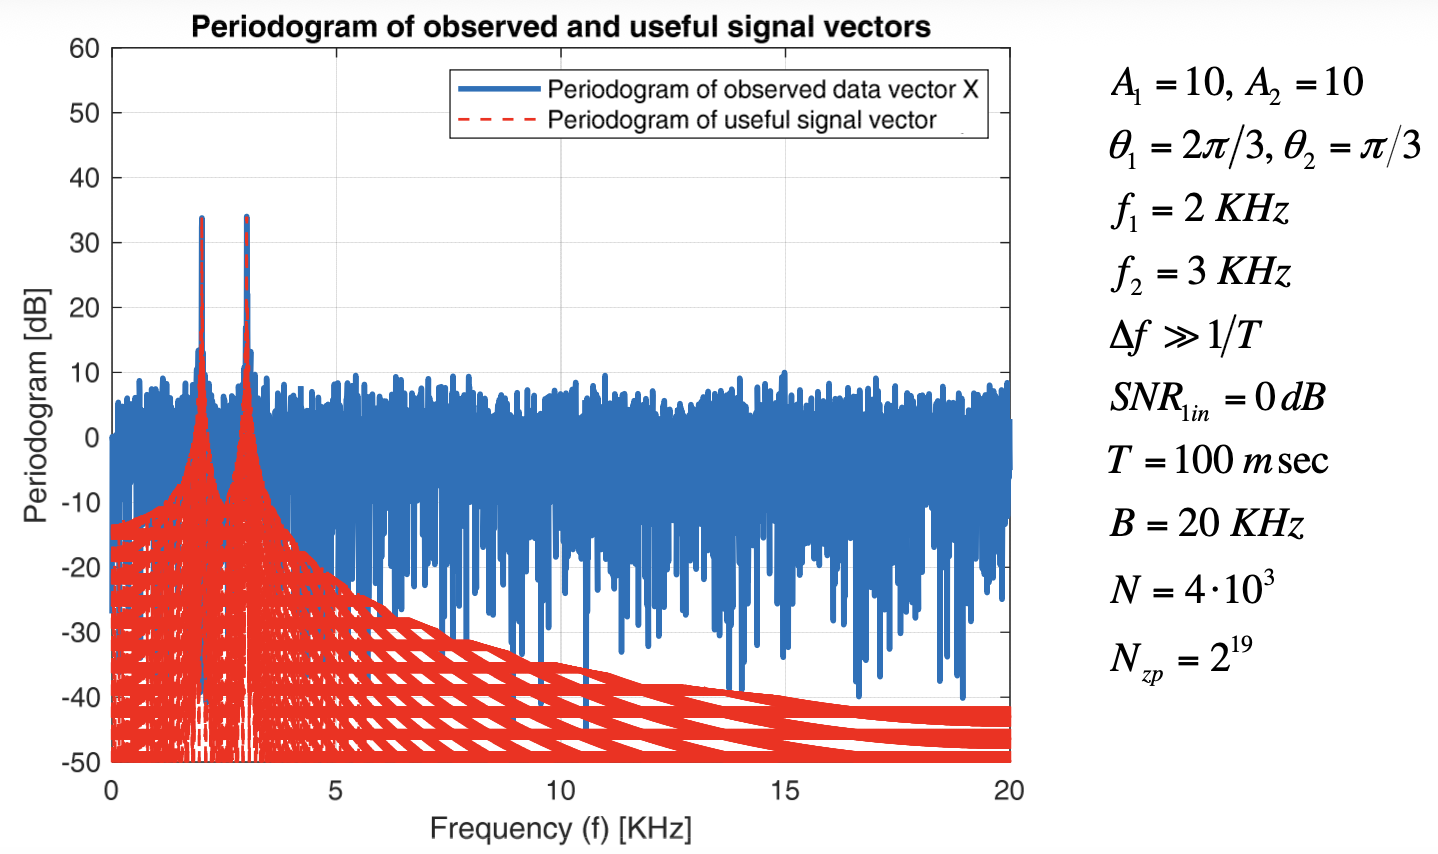
\includegraphics[width=0.6\linewidth]{Image/pdf 4/58.Period_signal.png}
        \label{fig:placeholder}
    \end{figure}
\begin{figure}[H]
    \centering
    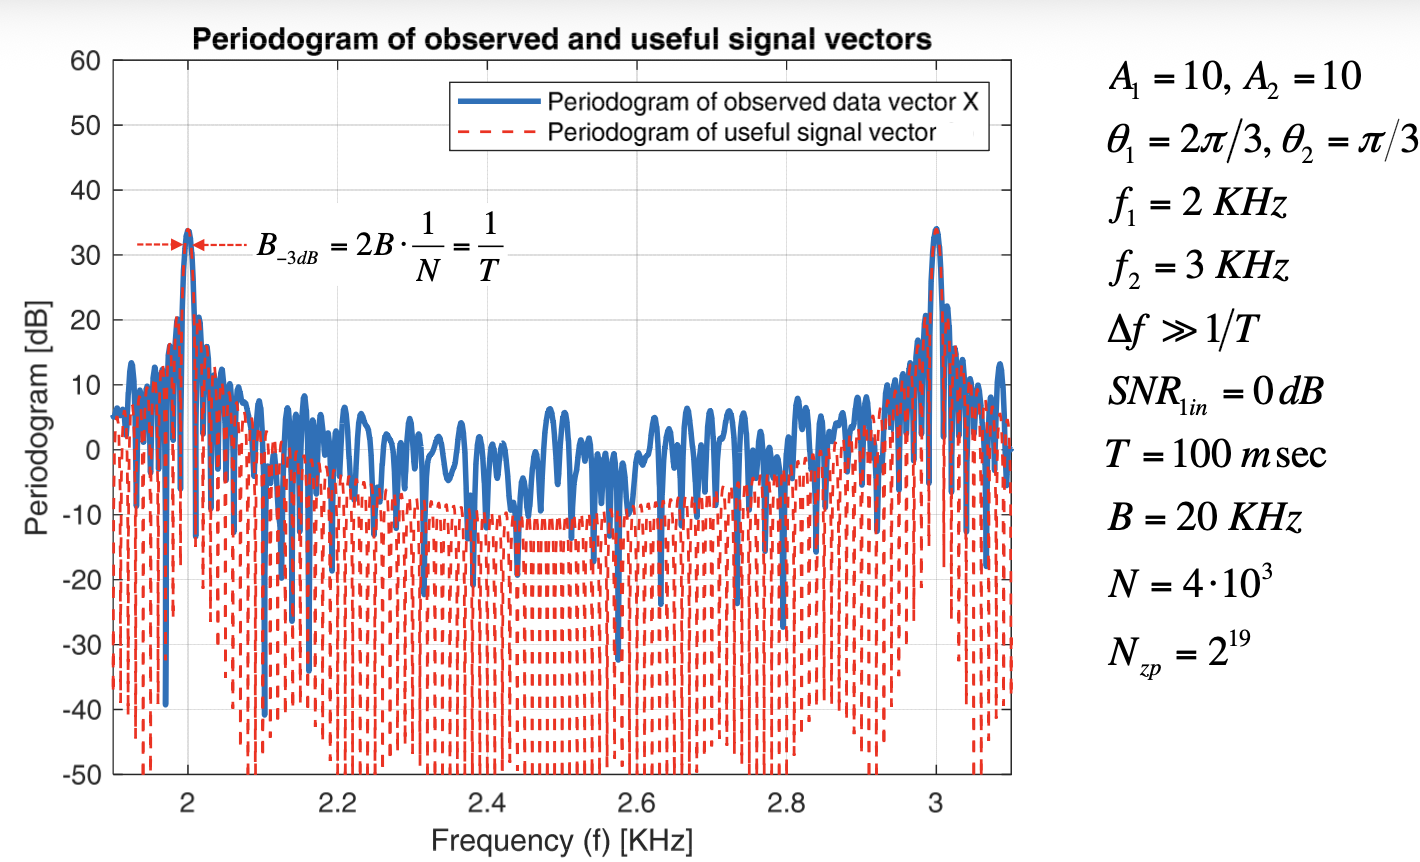
\includegraphics[width=0.6\linewidth]{Image/pdf 4/59.Period_sign_2.png}
    \label{fig:placeholder}
\end{figure}
\begin{figure}[H]
    \centering
    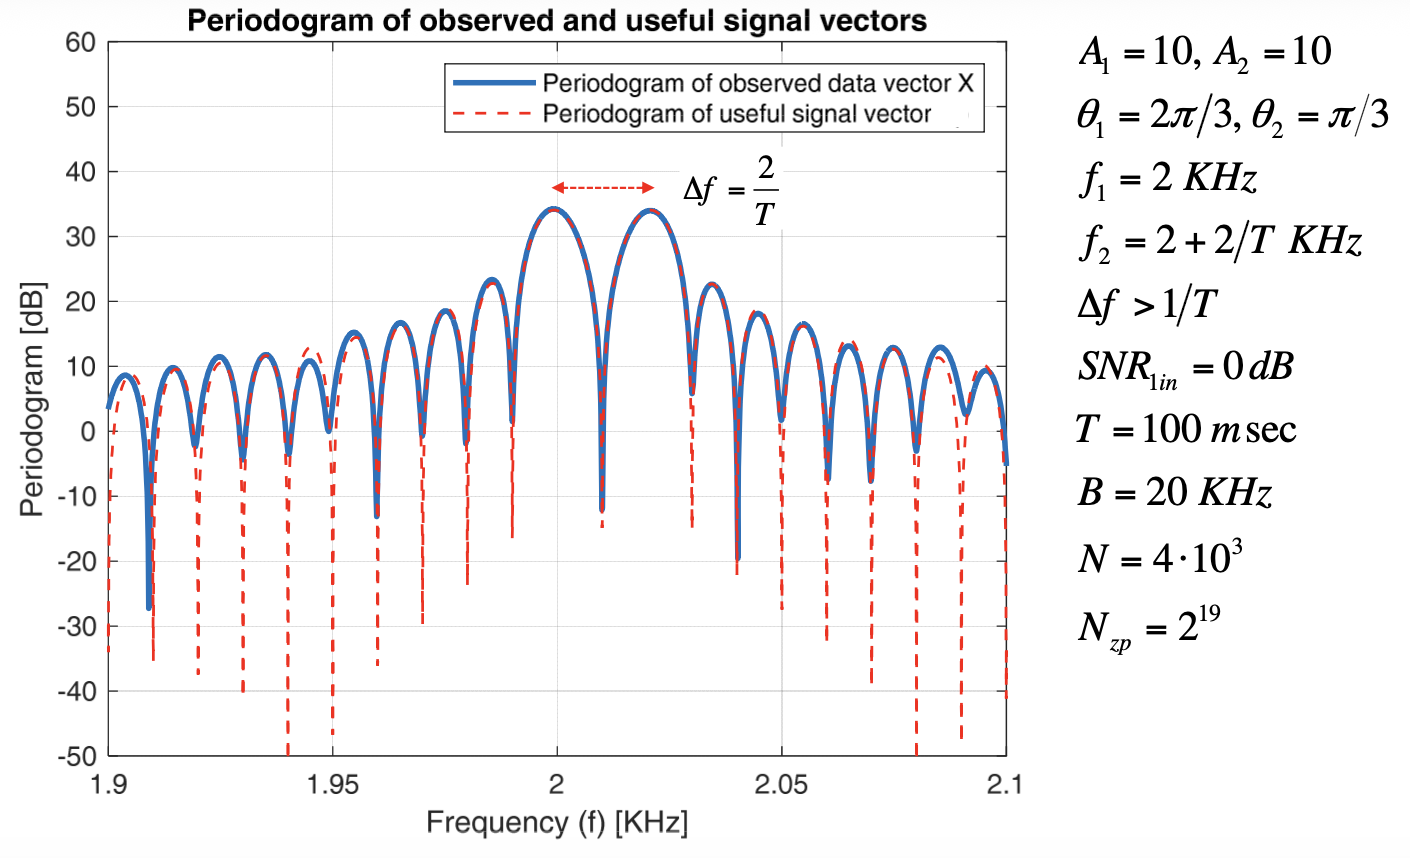
\includegraphics[width=0.6\linewidth]{Image/pdf 4/60.Period_sign_3.png}
    \label{fig:placeholder}
\end{figure}
\begin{figure}[H]
    \centering
    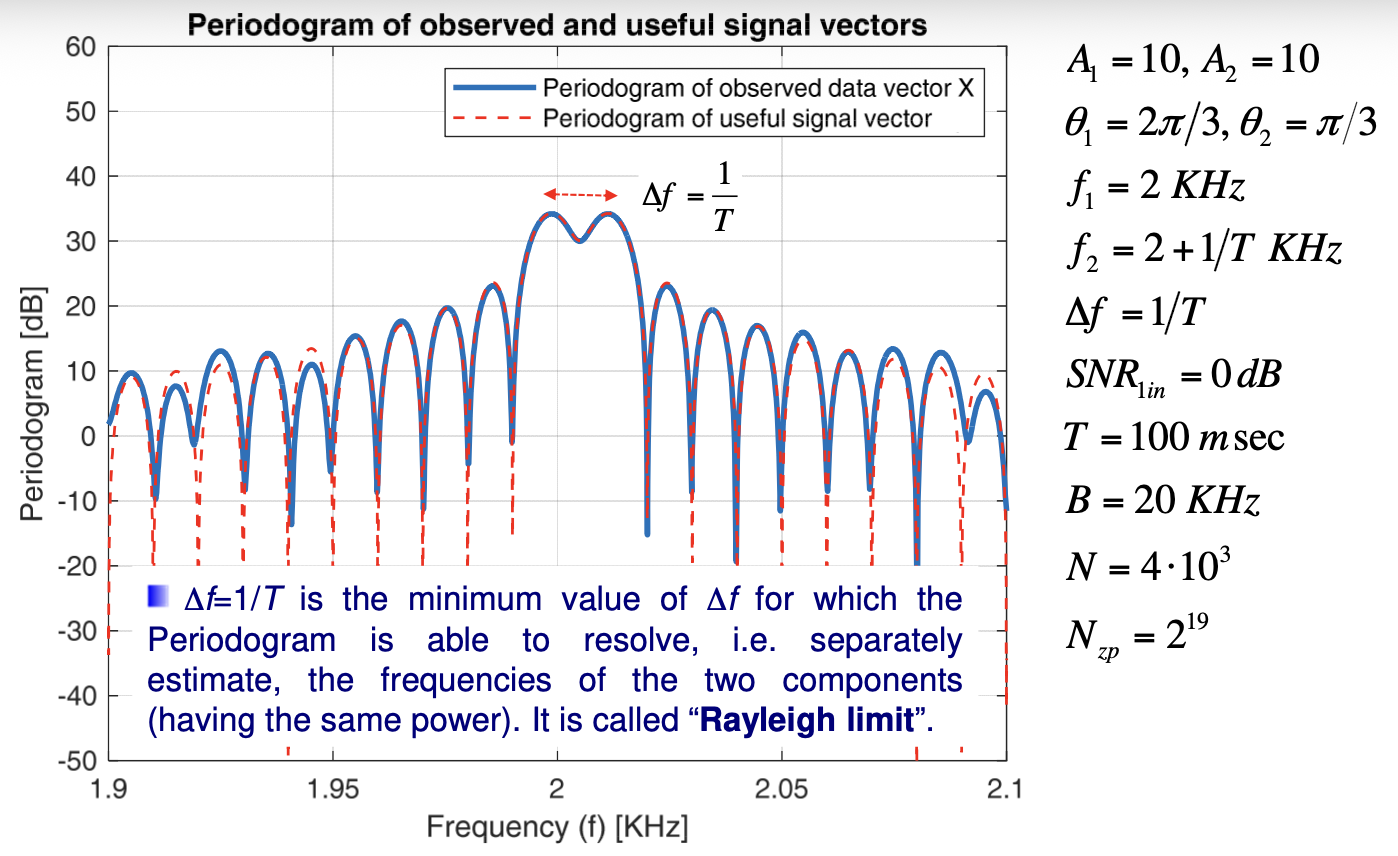
\includegraphics[width=0.6\linewidth]{Image/pdf 4/61.Period_sign_4.png}
    \label{fig:placeholder}
\end{figure}
\begin{figure}[H]
    \centering
    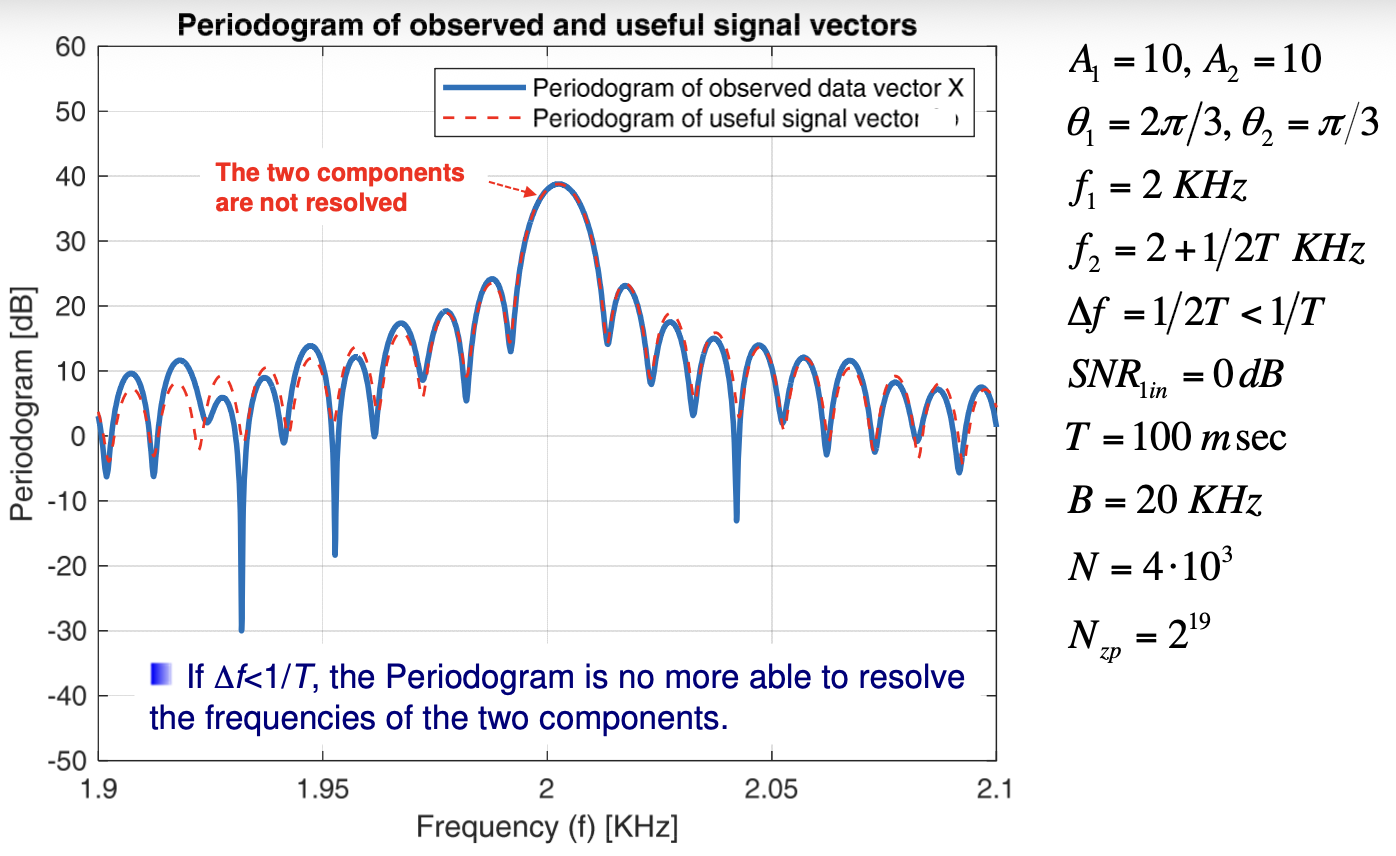
\includegraphics[width=0.6\linewidth]{Image/pdf 4/62.Period_sign_5.png}
    \label{fig:placeholder}
\end{figure}
\begin{figure}
    \centering
    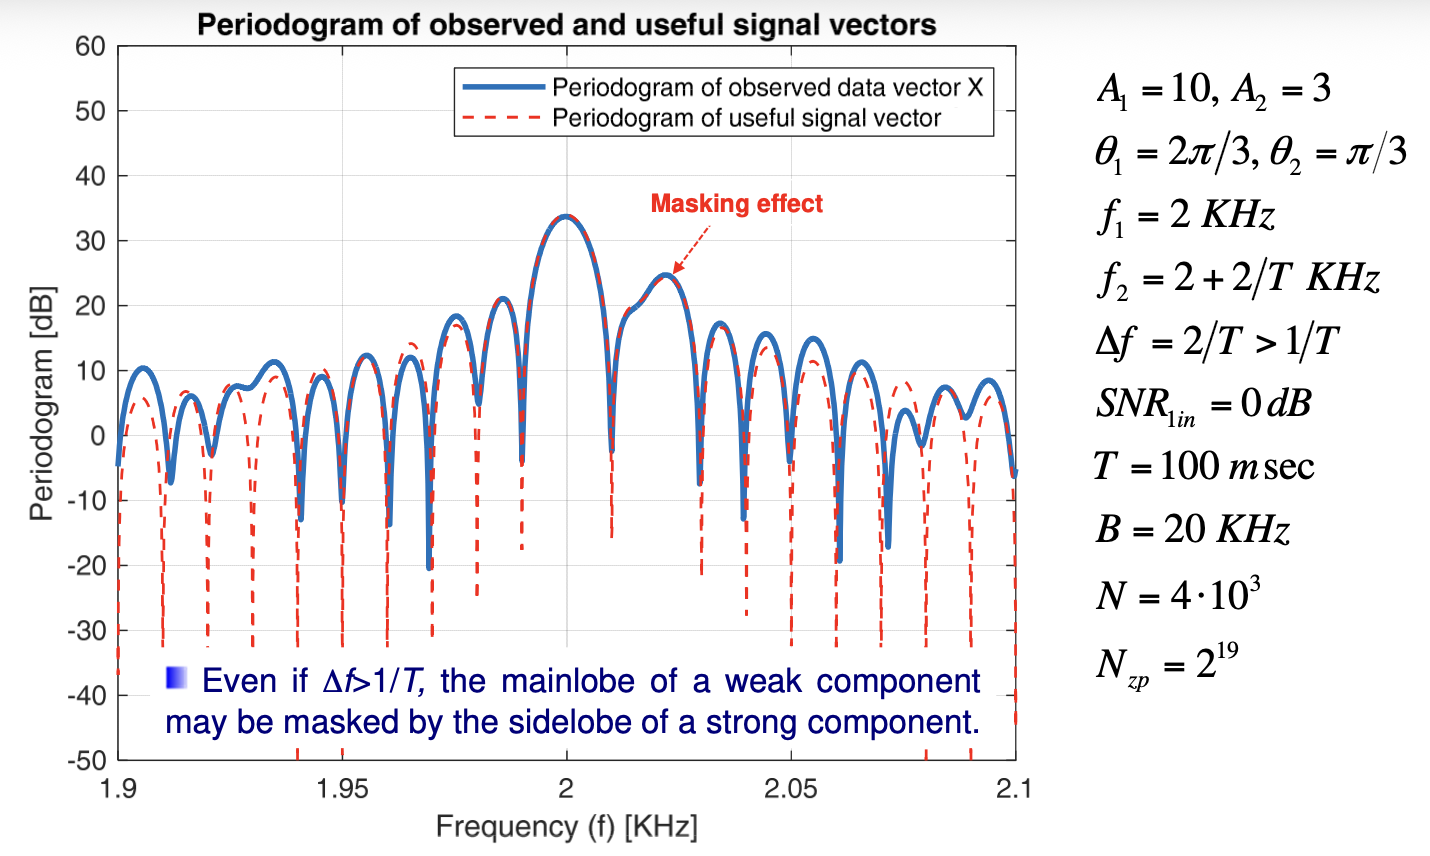
\includegraphics[width=0.6\linewidth]{Image/pdf 4/63.Period_sign_6.png}
    \label{fig:placeholder}
\end{figure}
\item \textbf{Resolution of the Periodogram}: \(\Delta f= 1/T\)(\textbf{Rayleigh limit})
\item To resolve multiple components that are separated by less than \(1/T\) (in the digital frequency domain the Rayleigh limit is \(1/N\)) we need to use "\textbf{superresolution methods}", e.g Nonlinear Least Squares.
\item Once we have estimated the frequencies of the various components we can estimate amplitudes and phases in the usual way, from the amplitude and phase of the Fourier Transform (FT) of the received signal at the estimated frequencies.
\end{itemize}
\subsection{Range/Time-Delay(TD) estimation}
Given \(s(t)\neq0\), \(\forall t\in[0,T_s)\) and \(X(t)=s(t-t_0)+W(t)\), \(t\in[0,T)\)
Find \(t_0=2R/c\), where \(c\) is the speed of propogation and \(R\) is the range \(W(t)\) AWGN: \(S_W(f)=\frac{N_0}{2}\)
\begin{itemize}
    \item The observation interval is of finite duration \(T\), long enough to contain the delayed version of the signal: \(T\geq T_s+t_0\).
    \item Given \(T,t_{max}=\max{t_0}=T-T_s\) and as a consequence \(R_{max}=\max{R}=c(T-T_s)/2\).
    \item Hence, given the \(R_{max}\) we want, we select \(T\) such that: \(T=T_s+T_{max}=T_s+2R_{max}/c\).
    \item As usual, we set \(B\) such that \(2BT\gg1\) and we filter the signal with a LTI low-pass filter (the anti-aliasing filter) with bandwidth \(B\) and then we sample at the Nyquist rate \(T_c=1/2B\).
    \[
X[n] = \frac{1}{\sqrt{2B}}\,X(t)\bigg|_{t = \frac{n}{2B}}
     = \frac{1}{\sqrt{2B}}\,s\!\left(\frac{n}{2B} - t_{0}\right)
       + \frac{1}{\sqrt{2B}}\,W\!\left(\frac{n}{2B}\right)
     = s[n - n_{0}] + W[n]
\]

where
\[
n_{0} = \left[ \frac{t_{0}}{1/(2B)} \right]
\]
is the delay in samples,
\[
N_{s} = \left[ \frac{T_{s}}{1/(2B)} \right]
\]
is the signal length in samples, and
\[
N = \left[ \frac{T}{1/(2B)} \right]
\]
is the observation interval in samples, i.e., the data size.
    \item Discrete-time data model:
\[
X[n] =
\begin{cases}
s[n-n_{0}] + W[n],
  & n \in [n_{0},\, n_{0}+N_{s}-1], \\[4pt]
W[n],
  & n \in [0,\, n_{0}-1] \cup [n_{0}+N_{s},\, N-1]
\end{cases}
\]

\[
\{W[n]\}_{n=0}^{N-1} \in \mathcal{N}\!\left(0,\sigma_{W}^{2}\right),
\quad \text{IID}, \qquad
\sigma_{W}^{2} = \frac{N_{0}}{2}
\]

\[
\{X[n]\}_{n=0}^{N-1} \ \text{mutually independent}, 
\qquad X_n \triangleq X[n], \quad s_n(n_0) \triangleq s[n-n_0]
\]

\[
f_X(\mathbf{x};n_0) = \prod_{n=0}^{N-1} f_{X_n}(x_n;n_0)
   = \prod_{n=0}^{N-1} \frac{1}{\sqrt{\pi N_0}}
   e^{-\frac{(x_n - s_n(n_0))^2}{N_0}}
   = (\pi N_0)^{-N/2} e^{-\frac{1}{N_0}\sum_{n=0}^{N-1}(x_n - s_n(n_0))^2}
\]

\[
\ln L(n_0) \triangleq \ln f_X(\mathbf{x};n_0)
  = \sum_{n=0}^{N-1} \ln f_{X_n}(x_n;n_0)
  = \kappa - \frac{1}{N_0} \sum_{n=0}^{N-1} (x_n - s_n(n_0))^2
\]

\[
\hat{n}_{0,ML}
  = \arg\max_{n_0} \ln L(n_0)
  = \arg\min_{n_0} \sum_{n=0}^{N-1} (x_n - s_n(n_0))^2
  = \arg\min_{n_0} \|\mathbf{x} - \mathbf{s}(n_0)\|^2
  = \hat{n}_{0,\text{NLLS}}
\]

\[
\sum_{n=0}^{N-1} (x_n - s_n(n_0))^2
  = \sum_{n=0}^{N-1} x_n^2
  + \sum_{n=0}^{N-1} s_n^2(n_0)
  - 2\sum_{n=0}^{N-1} x_n s_n(n_0)
  = E_X + E_S - 2E_{XS}(n_0)
\]
\[
\hat{n}_{0ML} = \underset{n_0}{\operatorname{arg\,min}} \sum_{n=0}^{N-1} \left( x_n - s_n(n_0) \right)^2 = 
\underset{n_0}{\operatorname{arg\,min}} \left( E_X + E_S - 2E_{XS}(n_0) \right) = 
\underset{n_0}{\operatorname{arg\,max}} E_{XS}(n_0)
\]
\item The ML estimate of \(n_0\) is the value that maximazes the mutual energy between the received data \(X[n]\) and \(s[n-n_0]\).
\[
E_{XS}(n_0)=\sum_{n = 0}^{N-1}x_ns_n(n_0)\quad \text{is an inner product, i.e. the matched filter output}
\]
\item We should implement a bank of LTI filters matched to \(s[n-n_0]\) for all possible values of \(n_0\) and select the value for which the MF output is maximal.
\item In practice, instead of implementing a bank of filters matched to \(s[n-n_0]\) for all possibile values of \(n_0\), this can be obtained by looking for the time \(N_{max}\) when the output of the filter matched to \(s[n]\) has the peak:
\[
\hat{n}_{0ML} = \underset{n_0}{\arg \max} E_{XS}(n_0) = N_{msx}-(N_s-1)
\]
\item For example, if \(s[n]\) is a rectangular pulse of length \(N_S\), i.e. from 0 to \(N_s-1\):
\begin{figure}[H]
    \centering
    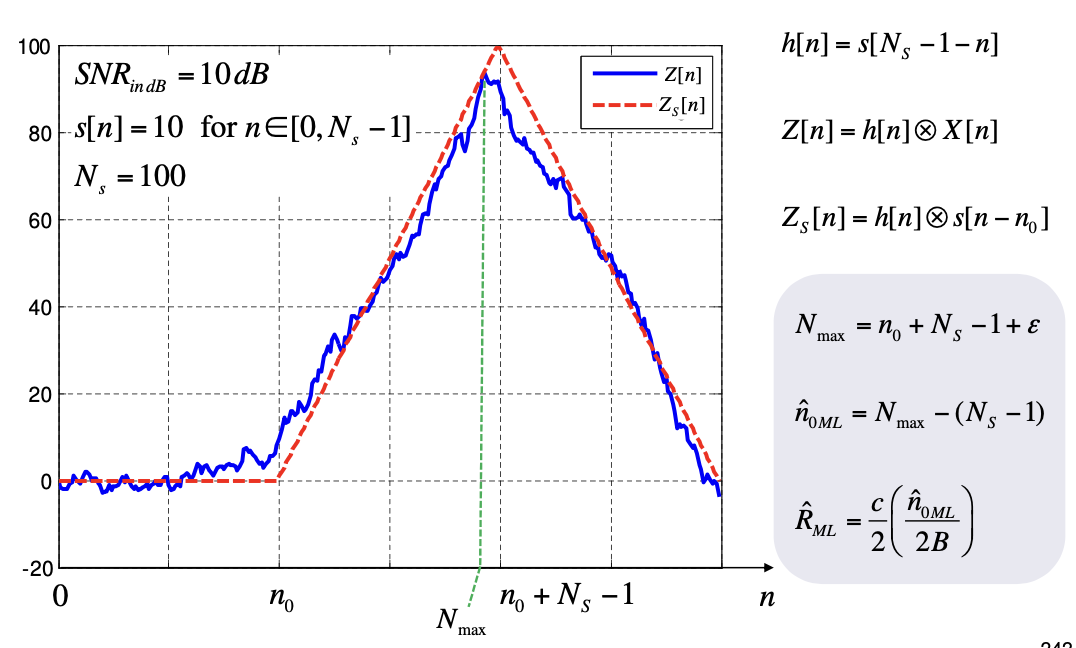
\includegraphics[width=0.6\linewidth]{Image/pdf 4/64.Time_delay.png}
    \label{fig:placeholder}
\end{figure}
\item CRB on the estimate of the Time Delay (TD) \(t_0\) and on the range \(R\):
\begin{align*}
\ln L(n_0) &\triangleq \ln f_X(\mathbf{x}; n_0) = \sum_{n=0}^{N-1} \ln f_{X_n}(x_n; n_0) = \kappa - \frac{1}{N_0} \sum_{n=0}^{N-1} (x_n - s_n(n_0))^2 \\
&= \kappa - \frac{1}{N_0} \|\mathbf{x} - \mathbf{s}(n_0)\|^2 = \kappa - \frac{1}{N_0} \int_0^T \left( x(t) - s(t-t_0) \right)^2 dt \triangleq \ln L(t_0) \\[2ex]
\frac{d \ln L(t_0)}{dt_0} &= \frac{2}{N_0} \int_0^T \left( x(t) - s(t-t_0) \right) \frac{ds(t-t_0)}{dt_0} dt \\[2ex]
\frac{d^2 \ln L(t_0)}{dt_0^2} &= \frac{2}{N_0} \int_0^T \left( x(t) - s(t-t_0) \right) \frac{d^2 s(t-t_0)}{dt_0^2} dt - \frac{2}{N_0} \int_0^T \left( \frac{ds(t-t_0)}{dt_0} \right)^2 dt
\end{align*}
\begin{align*}
I(t_0) &= -E\left\{\frac{d^2 \ln L(t_0)}{dt_0^2}\right\} = \frac{2}{N_0} \int_0^T \left(\frac{d s(t-t_0)}{dt_0}\right)^2 dt \\[2ex]
MSE\left\{\hat{t}_{0ML}\right\} &\geq CRB(t_0) = \frac{1}{I(t_0)} = \frac{N_0/2}{\int_0^T \left(\frac{d s(t-t_0)}{dt_0}\right)^2 dt} 
= \frac{N_0/2}{\int_{t_0}^{t_0+T_s} \left(\frac{d s(t-t_0)}{dt_0}\right)^2 dt} 
= \frac{N_0/2}{\int_0^{T_s} \left(\frac{d s(t)}{dt}\right)^2 dt} \\[2ex]
&= \frac{N_0/2}{\int_{-\infty}^{+\infty} |j 2\pi f \cdot S(f)|^2 df}
= \frac{N_0/2}{E_S \bar{\beta}^2} \\[2ex]
\bar{\beta}^2 &\triangleq \frac{\int_{-\infty}^{+\infty} |2\pi f \cdot S(f)|^2 df}{\int_{-\infty}^{+\infty} |S(f)|^2 df}
= \frac{\int_{-\infty}^{+\infty} (2\pi f)^2 |S(f)|^2 df}{E_S}
\end{align*}
    \[
n_0 = \left\lceil \frac{t_0}{1/2B} \right\rceil, \qquad
R = \frac{c}{2} t_0, \qquad
\mathrm{SNR} \triangleq \frac{E_s}{\sigma_w^2} = \frac{E_s}{N_0 / 2}, \qquad
\hat{R}_{ML} = \frac{c}{2} \hat{t}_{0ML} = \frac{c}{2} \left( \frac{\hat{n}_{0ML}}{2B} \right)
\]
\begin{align*}
\mathrm{MSE}\left\{ \hat{t}_{0ML} \right\} &\geq \mathrm{CRB}(t_0) = \frac{N_0 / 2}{E_s \beta^2} = \frac{1}{\mathrm{SNR} \cdot \beta^2}\\[3pt]
\mathrm{MSE}\left\{ \hat{R}_{ML} \right\} &\geq \mathrm{CRB}(R) = \frac{c^2}{4} \cdot \mathrm{CRB}(t_0) = \frac{c^2}{4 \mathrm{SNR} \cdot \beta^2}
\end{align*}
    \item We observe that the \textbf{range estimation accuracy} improves with the \textbf{bandwidth} of the transmitted signal, and obviously also with the SNR.
    \item This CRB does not take the \textbf{quantization error} (due to the temporal sampling) into account; in other words, due to the fact that \(t_0/(1/2B)\) in general is not an integer number.
    \item The are many methods to increase the \textbf{bandwidth} without reducing the pulse length \(T_s\)(since reducing \(T_s\) would imply reducing \(E_s\)).
    \item The most widely adopted method is to use a \textbf{Linearly Frequency Modulated(LFM)} waveform.
    \item The waveform is commonly referred to as a "\textbf{chirp}" waveform because a similar pulse in the audible frequency range produces a chirping sound.
    \item The basic idea is to sweep the frequency band \(B_s\) linearly during the pulse length \(T_s\). as shown in the next page.
    \item A narrowband \textbf{linear-FM(LFM)} pulse of energy \(E_s\) is given by:
\[
s(t) = \sqrt{\frac{2E_s}{T_s}} \cdot \cos\left(2\pi f_0 t + \pi k t^2 \right) \cdot \mathrm{rect}\left(\frac{t}{T_s}\right), \qquad \text{where} \quad k = \pm \frac{B_s}{T_s}
\]
    \item if \(k\) is positive, the pulse is an \textit{upchirp}, if negative its is a \textit{downchirp}.
    \begin{figure}[H]
        \centering
        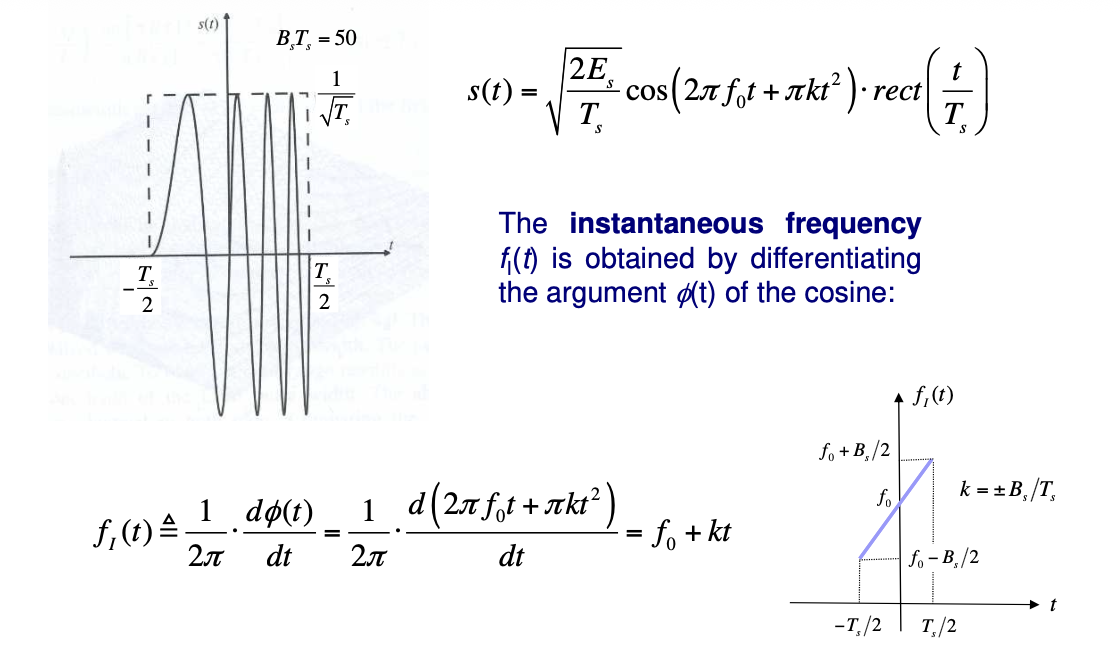
\includegraphics[width=0.6\linewidth]{Image/pdf 4/65.Foto.png}
        \label{fig:placeholder}
    \end{figure}
    \item \underline{The instantaneous frequency is a linear function of time}.
    \item For low \(B_sT_s\), the spectrum is relatively poorly defined.
    \item As the \(B_sT_s\) product increases, the spectrum takes on more rectangular shape (around the central frequency \(f_0\)). This is intuitively reasonable, because the sweep is linear, the waveform spreads its energy uniformly across the spectrum.
\begin{figure}[H]
    \centering
    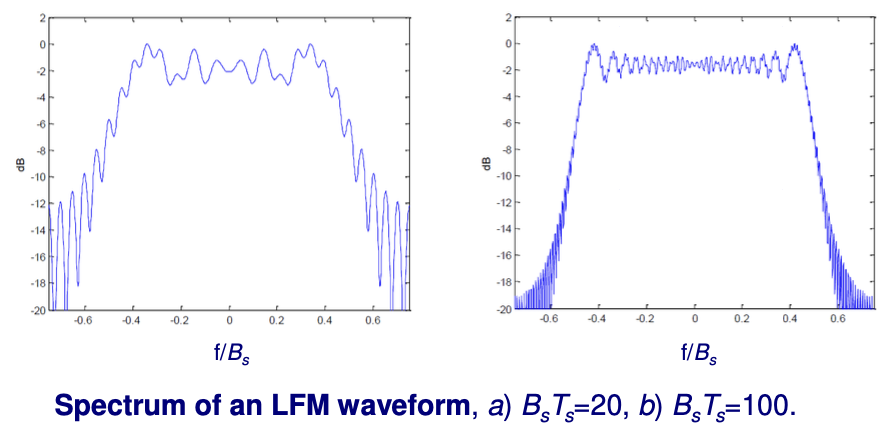
\includegraphics[width=0.6\linewidth]{Image/pdf 4/66.LFM.png}
    \label{fig:placeholder}
\end{figure}
\end{itemize}
\subsection{Signal Estimation in Gaussian/Laplace Noise}
\begin{itemize}
    \item \textbf{Problem}: We observe \(N\) samples of a realization of the discrete-time rando process \(X[n]=A+W[n]\), for \(n=0,1,2,\cdots,N-1\), where the SOI \(A\) is modelled as an unknown deterministic parameter and \(\{W[n]\}\) are independent and IID zero mean random variable with symmetric distribution, modelling the additive noise. The noise power is also unknown.
\[
\mathbf{X}_{N \times 1} = 
\begin{bmatrix} 
\mathrm{X}[0] & \mathrm{X}[1] & \cdots & \mathrm{X}[N-1]
\end{bmatrix}^T, 
\qquad 
\left\{ X_i \right\}_{i=0}^{N-1} \ \text{\textbf{IID}}
\]

\[
m_1 = E\{X_i\} = \mathrm{median}\{X_i\} = A, \qquad
\mu_2 = \mathrm{var}\{X_i\} = \textit{noise power}
\]

    \item When the noise samples are modelled as zero mean \textbf{Gaussian} r.v.s with variance \(\sigma^2\), we know that the \textbf{Maximum Likelihood (ML)} estimators of \(A\)(the mean of \(X[n]\)) and \(\sigma^2\) (the variance of \(X[n]\)) are given by the \textbf{sample mean} and the \textbf{sample variance} of the observed data, and they coincide with the \textbf{MM} estimators.
\[
\mathbf{X}_{N \times 1} = \begin{bmatrix} X[0] & X[1] & \cdots & X[N-1] \end{bmatrix}^{T}, \qquad \{ X_n \}_{n=0}^{N-1} \;\text{IID}
\]

\[
\text{Gaussian noise:} \qquad f_{X_n}(x_n) = \frac{1}{\sqrt{2\pi\sigma^2}} \exp \left( -\frac{(x_n - A)^2}{2\sigma^2} \right), \qquad n = 0,1,\ldots,N-1
\]

\[
\rightarrow \quad m_1 = \mathbb{E}\{ X_n \} = \operatorname{median}\{X_n\} = A, \qquad \mu_2 = \operatorname{var}\{ X_n \} = \sigma^2
\]

\[
\left\{
\begin{array}{l}
A = m_1 = \mathbb{E}\{ X[n] \} \\[1ex]
\sigma^2 = \mu_2 = \mathbb{E}\{ ( X[n] - A )^2 \}
\end{array}
\right.
\qquad \implies \qquad
\left\{
\begin{array}{l}
\hat{A}_{ML} = \hat{A}_{MM} = \hat{m}_1 = \frac{1}{N} \sum_{n=0}^{N-1} x[n] \\[2.5ex]
\hat{\sigma}^2_{ML} = \hat{\sigma}^2_{MM} = \hat{\mu}_2 = \frac{1}{N} \sum_{n=0}^{N-1} \left( X[n] - \hat{m}_1 \right)^2
\end{array}
\right.
\]
    
    \item \underline{Let us now investigate the case where the noise is \textbf{non Gaussian} and should be modelled by an }\\
    \noindent \underline{heavy-tailed distribution, e.g. the \textbf{Laplace} distribution}:
    \[
\text{Laplace noise:} \quad
f_{X_n}(x_n) = \frac{1}{2\eta} \exp\left(-\frac{|x_n - A|}{\eta}\right),
\quad n = 0, 1, \ldots, N-1
\]

\[
\rightarrow \quad
m_1 = \mathbb{E}\{ X_n \} = \operatorname{median}\{ X_n \} = A, \qquad
\mu_2 = \operatorname{var}\{ X_n \} = 2\eta^2
\]
    \item The \textbf{MM} estimators are the same as in the Gaussian case, i.e. they are the \textbf{sample mean} and \textbf{sample variance}:
\[
\left\{
\begin{array}{l}
\hat{A}_{MM} = \hat{m}_1 = \frac{1}{N} \sum\limits_{n=0}^{N-1} X[n] \\[3ex]
2\hat{\eta}^2_{MM} = \hat{\mu}_2 = \frac{1}{N} \sum\limits_{n=0}^{N-1} \left( X[n] - \hat{m}_1 \right)^2
\end{array}
\right.
\implies
\hat{\eta}_{MM} = \sqrt{ \frac{1}{2N} \sum\limits_{n=0}^{N-1} \left( X[n] - \hat{m}_1 \right)^2 }
\]

    \item However, remember that the \textbf{sample} estimators, the \textbf{MM} estimators, and the \textbf{ML} estimators coincide only if the additive noise is white \textbf{Gaussian} distributed.
    \item The \textbf{bias} and the \textbf{MSE} of the \textbf{MM estimator} of \(A\) in Laplace noise are given by:
\[
E\{\hat{A}_{MM}\} = \frac{1}{N} \sum_{n=0}^{N-1} E\{X[n]\}
= \frac{1}{N} \sum_{n=0}^{N-1} A = A
\qquad \rightarrow \quad \text{the MM estimator is unbiased}
\]

\[
MSE\{\hat{A}_{MM}\} = \mathrm{var}\{\hat{A}_{MM}\}
= \mathrm{var}\left\{ \frac{1}{N} \sum_{n=0}^{N-1} X[n] \right\}
= \frac{1}{N^2} \, \mathrm{var}\left\{ \sum_{n=0}^{N-1} X[n] \right\}
\]

\[
= \frac{1}{N^2} \sum_{n=0}^{N-1} \mathrm{var}\{X[n]\}
= \frac{1}{N^2} \sum_{n=0}^{N-1} E\{W^2[n]\}
= \frac{2\eta^2}{N}
\]

\[
\rightarrow \quad \text{the MM estimator is consistent}
\]

    \item The bias and the MSE of the MM estimator of \(\eta\) cannot be derived analytically.
    \item \underline{Let us now derive the \textbf{ML estimators} of \(A\) and \(\eta\) when the noise is \textbf{Laplace} distributed}:
\[
\text{Laplace noise:} \quad
f_{x_n}(x_n) = \frac{1}{2\eta} e^{-\frac{|x_n - A|}{\eta}},
\qquad n = 0, 1, \cdots, N-1, \quad \text{IID}
\]

\[
f_{\mathbf{X}}(\mathbf{x}; A, \eta) = \prod_{n=0}^{N-1} f_{X}(x_n; A,\eta)
= \left( \frac{1}{2\eta} \right)^N
\exp \left( -\frac{1}{\eta} \sum_{n=0}^{N-1} |x_n - A| \right)
\]

\[
\ln LF(A, \eta) = \ln f_{\mathbf{X}}(\mathbf{x};A,\eta)
= -N \ln(2) - N \ln(\eta) - \frac{1}{\eta} \sum_{n=0}^{N-1} |x_n - A|
\]


    \item The ML estimators is derived by solving the \textbf{likelihood equation}.
\[
\frac{d\ln LF(A, \eta)}{dA} =
- \frac{1}{\eta} \cdot \frac{d}{dA} \left( \sum_{n=0}^{N-1} |x_n - A| \right)
= \frac{1}{\eta} \sum_{n=0}^{N-1} \mathrm{sign}(x_n - A) = 0
\]

\[
\sum_{n=0}^{N-1} \mathrm{sign}(x_n - A) = 0 
\]
    \item The value of \(A\) such that the ML equation is satisfied is given by the \textbf{Sample Median} of the data, i.e. we order the data vector \textbf{X}, e.g. with increasing order, and we select the median value. Assuming that \(N\) is an odd integer number, the median value is the sample at position \((N-1)/2\):
\[
\hat{A}_{ML} = \mathrm{median}\{\mathbf{X}\}
= Y\left[\frac{N-1}{2}\right]
\qquad \textit{Sample Median}
\]
\item Where \textbf{Y} is the ordered data vector such that \(Y[0]\leq Y[1]\leq\cdots \leq Y[N-2]\leq Y[N-1]\)
\item The ML estimator of \(A\) in Laplace noise does not require knowledge of the parameter \(\eta\), i.e. they are decoupled; it is \textbf{nonlinear} and requires an ordering of the data vector, so the computational complexity is higher than that of the MM estimator, which is linear.
\item Now, \underline{let us derive the ML estimator of the parameter \(\eta\)}, which provides the ML estimator of the noise power : \(\hat{\mu}_{2ML}=2\hat{\eta}^2_{ML}\)
\[
\frac{d \ln LF(A, \eta)}{d\eta}
= -\frac{N}{\eta}
+ \frac{1}{\eta^2} \sum_{n=0}^{N-1} |x_n - A|
= 0
\]

\[
\eta = \frac{1}{N} \sum_{n=0}^{N-1} |x_n - A|
\qquad \rightarrow \qquad
\hat{\eta}_{ML} = \frac{1}{N} \sum_{n=0}^{N-1} |x_n - \hat{A}_{ML}|
\]
\item Which is the so-called \textbf{Mean Absolute Deviation (MAD from the Median.}
\item To derive analytically the \textbf{bias} and the \textbf{MSE} of the \textbf{ML estimator} of \(A\) and \(\eta\) in \textbf{Laplace noise} is a very difficul task.
\item We can derive bias and MSE of the ML estimators by Monte Carlo simulation.
\item Let us derive the \textbf{Cramèr-Rao lower bounds (CRB)} for \(A\) and \(\eta\), which provide the asymptotic MSE of the ML estimators:
\[
\frac{d^2 \ln LF(A, \eta)}{dA^2} =
\frac{d}{dA} \left( \frac{d \ln LF(A, \eta)}{dA} \right)
= \frac{1}{\eta} \sum_{n=0}^{N-1} \frac{d}{dA} \, \big(\, \mathrm{sign}(x_n - A)\, \big)
= -\frac{2}{\eta} \sum_{n=0}^{N-1} \delta(x_n - A)
\]

\begin{align*}
I_{11} &= -E\left\{ \frac{d^2 \ln LF(A, \eta)}{dA^2} \right\}
= -E\left\{ -\frac{2}{\eta} \sum_{n=0}^{N-1} \delta(x_n - A) \right\}
= \frac{2}{\eta} \sum_{n=0}^{N-1} \left[
    \int_{-\infty}^{+\infty} \delta(x_n - A) f_X(x_n) dx_n
\right]\\
&= \frac{2}{\eta} \sum_{n=0}^{N-1} f_X(A)
= \frac{2N}{\eta} f_X(A)
= \frac{2N}{\eta} \cdot \frac{1}{2\eta}
= \frac{N}{\eta^2}
\end{align*}
\begin{align*}
\frac{d^2 \ln LF(A, \eta)}{d \eta^2}
&= \frac{d}{d \eta} \left( \frac{d \ln LF(A, \eta)}{d \eta} \right)
= \frac{d}{d \eta}
\left( -\frac{N}{\eta} + \frac{1}{\eta^2} \sum_{n=0}^{N-1} |x_n - A| \right)\\
&= \frac{N}{\eta^2} - \frac{2}{\eta^3} \sum_{n=0}^{N-1} |x_n - A|\\
I_{22} &= -E\left\{ \frac{d^2 \ln LF(A, \eta)}{d \eta^2} \right\}
= -\frac{N}{\eta^2} + \frac{2}{\eta^3} \sum_{n=0}^{N-1} E\left\{ |x_n - A| \right\}
\end{align*}

\item We know that if \(X-\text{Laplace}(A,\eta)\) then \(Y = |X-A|\sim \text{Exp}(1/\eta)\), i.e.
\begin{align*}
f_X(x) &= \frac{1}{2\eta} e^{-\frac{|x - A|}{\eta}}
\qquad
Y = |x - A|
\implies
f_Y(y) = \frac{1}{\eta} e^{-\frac{y}{\eta}} u(y),\qquad E\{Y\} = \eta\\
I_{22} &= -\frac{N}{\eta^2}
+ \frac{2}{\eta^3} \sum_{n=0}^{N-1} E\{|x_n - A|\}
= -\frac{N}{\eta^2}
+ \frac{2N\eta}{\eta^3}
= \frac{N}{\eta^2}
\end{align*}
\begin{align*}
\frac{d^2 \ln LF(A,\eta)}{dA d\eta}
&= \frac{d}{dA} \left( \frac{d \ln LF(A,\eta)}{d\eta} \right) \\
&= \frac{d}{dA} \left(-\frac{N}{\eta} + \frac{1}{\eta^2} \sum_{n=0}^{N-1} |x_n - A| \right) \\
&= -\frac{1}{\eta^2} \sum_{n=0}^{N-1} \mathrm{sign}(x_n - A)
\end{align*}

\begin{align*}
I_{12} &= -E\left\{ \frac{d^2 \ln LF(A,\eta)}{dA d\eta} \right\} \\
&= \frac{1}{\eta^2} \sum_{n=0}^{N-1} E\left\{ \mathrm{sign}(x_n - A) \right\} \\
&= \frac{1}{\eta^2} \sum_{n=0}^{N-1} \left[ 1 \cdot \Pr\{x_n > A\} + (-1) \cdot \Pr\{x_n < A\} \right] \\
&= \frac{1}{\eta^2} \sum_{n=0}^{N-1} \left[ \frac{1}{2} - \frac{1}{2} \right] = 0
\end{align*}
\item Hence, FIM is diagonal and the two parameters are \underline{decoupled}.
\item The CRBs on the estimate of parameters \(A\) and \(\eta\) are given by:
\[
CRB(A)=\frac{1}{I_{11}}=\frac{\eta^2}{N}, \qquad CRB (\eta)=\frac{1}{I_{22}}=\frac{\eta^2}{N}
\]
\item Remember that:
\[
MSE\{\hat{A}_{MM}\} = \frac{2\eta^2}{N}=2\cdot CRB(A)
\]
\item So the MM estimator is not efficient, it is no even asymptotically efficient; whereas we know that the ML estimator is always asymptotically efficient. Hence, asymptotically (\(N\gg1\)) we have:
\[
MSE\{\hat{A}_{ML}\}=CRB(A)=\frac{\eta^2}{N}=\frac{MSE\{\hat{A}_{MM}\}}{2}
\] 

\item \textbf{Summary on the estimate of A}
    \begin{itemize}
        \item \textbf{Gaussian Noise} \textbf{Sample estimator = MM estimator = ML estimator}
        \item Mean value = Median = \(A\) \(\rightarrow\) we can use both the Sample Mean and the Sample Median to estimate \(A\)(the Sample Median is not the ML estimate, it is more robust to the presence of outliers, but it has higher computational complexity and higher MSE).
        \item \textbf{Laplace Noise}: \textit{Sample estimator} = \textit{MM estimator} \(\neq\) \textit{ML estimator}.\\
        Mean value = Media = \(A\) \(\rightarrow\) we can use both the Sample Mean and the Sample Median to estimate \(A\)(the Sample Median is the ML estimate, it has higher computational complexity but lower MSE; the Sample Mean is the MM estimate but not the ML estimate and it has higher MSE than the ML).
        
    \end{itemize}
    \item \textbf{\underline{Estimate of A - Sample Mean vs Sample Median}}
    \begin{figure}[H]
        \centering
        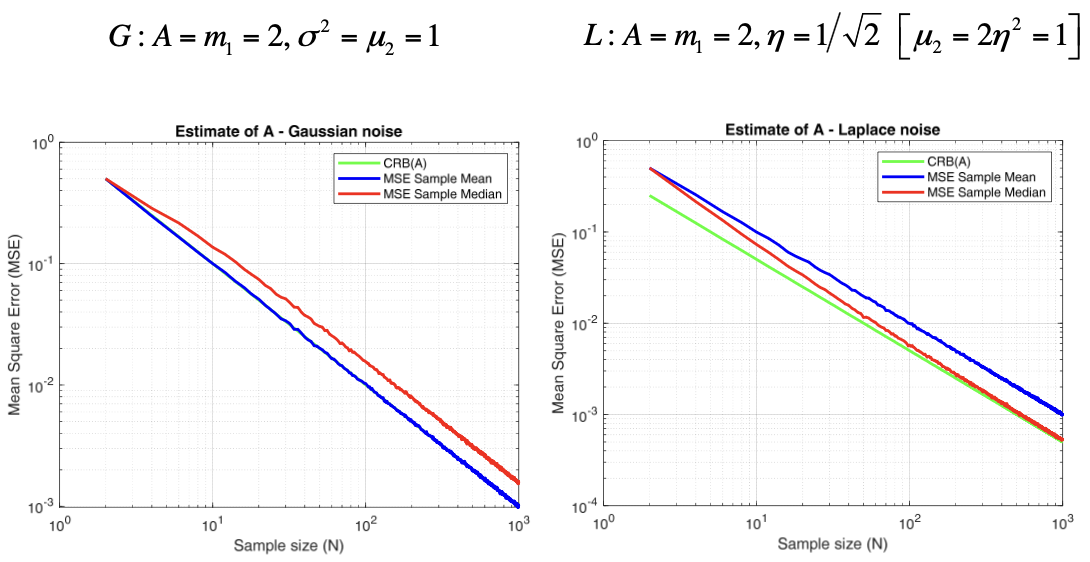
\includegraphics[width=0.6\linewidth]{Image/pdf 4/67.Penultimo.png}
        \label{fig:placeholder}
    \end{figure}
    \item \textbf{\underline{Estimate of \(\eta\)- Mean Absolute Deviation (MAD) from the Median}}
    \begin{figure}[H]
        \centering
        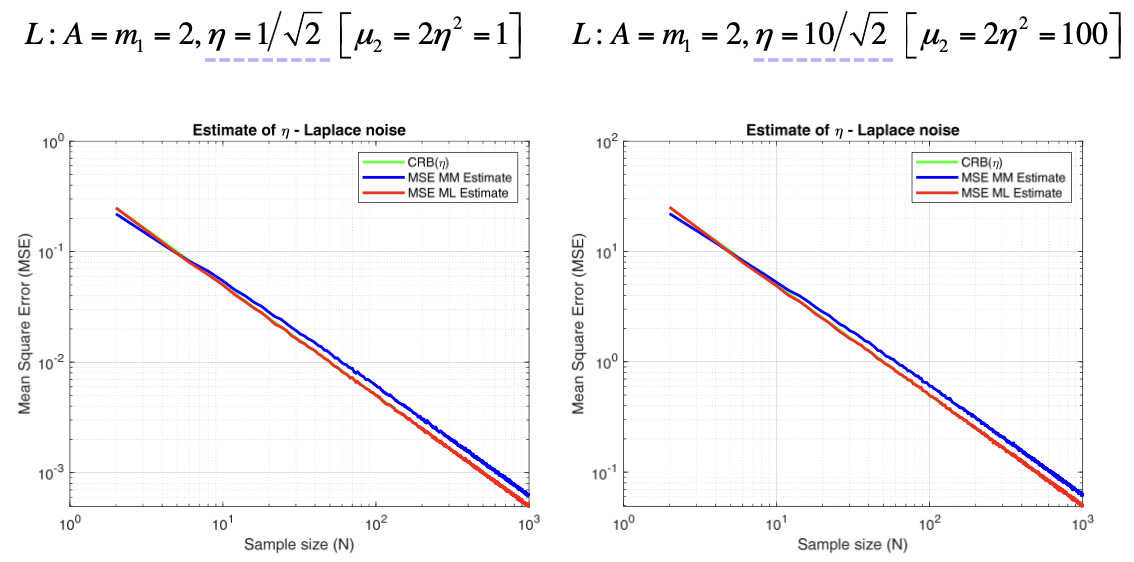
\includegraphics[width=0.6\linewidth]{Image/pdf 4/68.Ultimo.png}
        \label{fig:placeholder}
    \end{figure}

\end{itemize}



\clearpage



